\documentclass{journal}
\usepackage{graphicx}
\usepackage{siunitx}
\usepackage{float}
\usepackage{caption}


\begin{document}
\title{AP Calculus Final Project}
\author{Joshua Morin-Baxter, Alan Zhu, Nathan Wiley, and George Hong}
\date{\today}

\maketitle

\part{Wind Velocity vs. Wind Angle}
\begin{figure}[H]
  \centering
  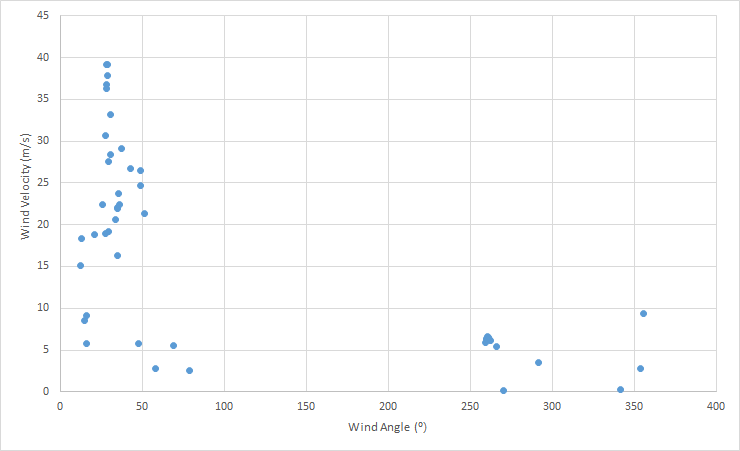
\includegraphics[width=\textwidth]{alan-data.png}
  \caption{Plot of Wind Velocity vs. Wind Angle}
\end{figure}

Although the tendencies of the data tend to wary between points, some overarching trends can be noted by analyzing the sign of the first and second derivatives (especially where they change).
The data can be analyzed on various intervals.
\begin{itemize}
  \item $angle \in (12^{\circ},16^{\circ})$: Data varies wildly.
  \item $angle \in (20^{\circ}, 28^{\circ})$ Data is almost consistently increasing, before reaching a critical point while being concave down (thus being a local maximum).
  \item $angle \in (29^{\circ}, 35^{\circ})$ Data is also almost consistently increasing.
  \item $angle \in (35^{\circ}, 37^{\circ})$ Data varies before reaching a critical point while being concave down (thus being a local maximum).
  \item $angle \in (37^{\circ}, 48^{\circ})$ Data slowly and inconsistently decreases.
  \item $angle \in (48^{\circ}, 52^{\circ})$ Decreases before reaching a critical point and point of inflection (thus being a local minimum)
  \item $angle \in (53^{\circ}, 80^{\circ})$ Data varies.
  \item $angle \in (259^{\circ}, 260.2^{\circ})$ Data is increasing and concave up before reaching a point of inflection
  \item $angle \in (260.2^{\circ}, 261^{\circ})$ Data is varying, but is critical and has a varying second derivative, meaning the data has a local maximum in this area.
  \item $angle \in (261^{\circ}, 271^{\circ})$ Data is decreasing, but second derivative goes from negative to positive, reaching a critical point where the second derivative is positive (thus being a local minimum)
  \item $angle \in (290^{\circ}, 355^{\circ})$ Data is consistently increasing, reaching a maximum at the end of the data.
\end{itemize}

The critical point on the interval $(35^{\circ}, 37^{\circ})$ and the general clustering of data around it represents the jet stream, blowing towards the NEbN (Northeast by North), while the critical point near 260 degrees seems to be the surface wind, which blows towards WbS (West by South).

The jet stream data can be fit by a normal distribution with $R = 0.536$.

\begin{figure}[H]
  \centering
  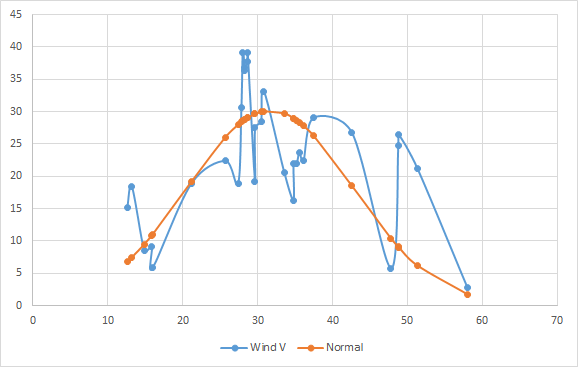
\includegraphics[width=\textwidth]{alan-data-2.png}
  \caption{Plot of Wind Velocity vs. Wind Angle on the Interval $(10^{\circ}, 60^{\circ})$ Fit by a Normal Distribution}
\end{figure}

\end{document}
